\section{Supplementary Information}
\appendix

\subsection{A) Tutorials, Code, and Documentation}
\label{app:tutorials}

\begin{itemize}


\item 
\href{https://colab.research.google.com/github/AIModelShare/aimodelshare_tutorials/blob/main/modelshareai/QST_Tabular_Classification.ipynb}{Tabular Classification Tutorial}

\item 
\href{https://colab.research.google.com/github/AIModelShare/aimodelshare_tutorials/blob/main/modelshareai/Keras_Image_Classification_Quick_Start_Tutorial.ipynb}{Image Classification Tutorial}

\item 
\href{https://colab.research.google.com/github/AIModelShare/aimodelshare_tutorials/blob/main/modelshareai/Text_Classification_QuickStart_IMDB.ipynb}{Text Classification Tutorial}

\item 
\href{https://colab.research.google.com/github/AIModelShare/aimodelshare_tutorials/blob/main/modelshareai/Keras_Video_Classification_Quick_Start_Tutorial(1).ipynb}{Video Classification Tutorial}

\item 
\href{https://www.modelshare.ai/notebooks/notebook:229}{Regression Tutorial}

\item 
\href{https://github.com/AIModelShare/aimodelshare}{Github Page}

\item 
\href{https://aimodelshare.readthedocs.io/en/latest/index.html}{Documentation}

\item 
\href{https://www.modelshare.ai/}{Modelshare AI Website}


\end{itemize}

\newpage
\subsection{B) Example of User Profile Page}
\label{app:profile_page}

\begin{figure}[h!]
  \centering
  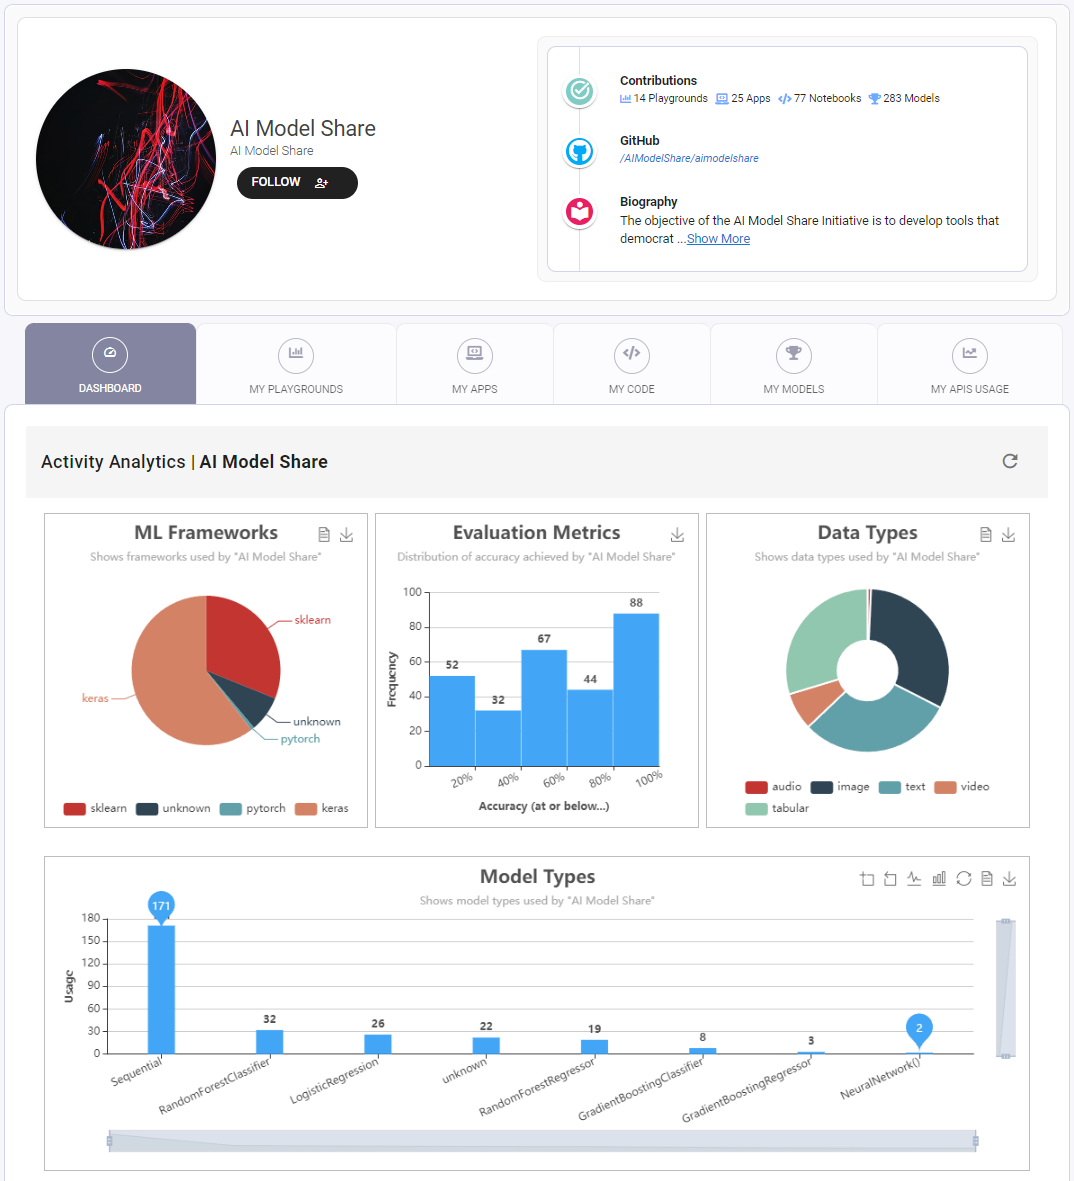
\includegraphics[width=1\textwidth]{figures/profile_page.png}
  \caption{Example of a user profile page. A User Profile Page shows aggregate information about a user's activity (Dashboard), and provides access to Model Playgrounds, apps, code, and models created by the user.}
\end{figure}

\newpage
\subsection{C) Example of Model Playground Page}
\label{app:playground}

\begin{figure}[h!]
  \centering
  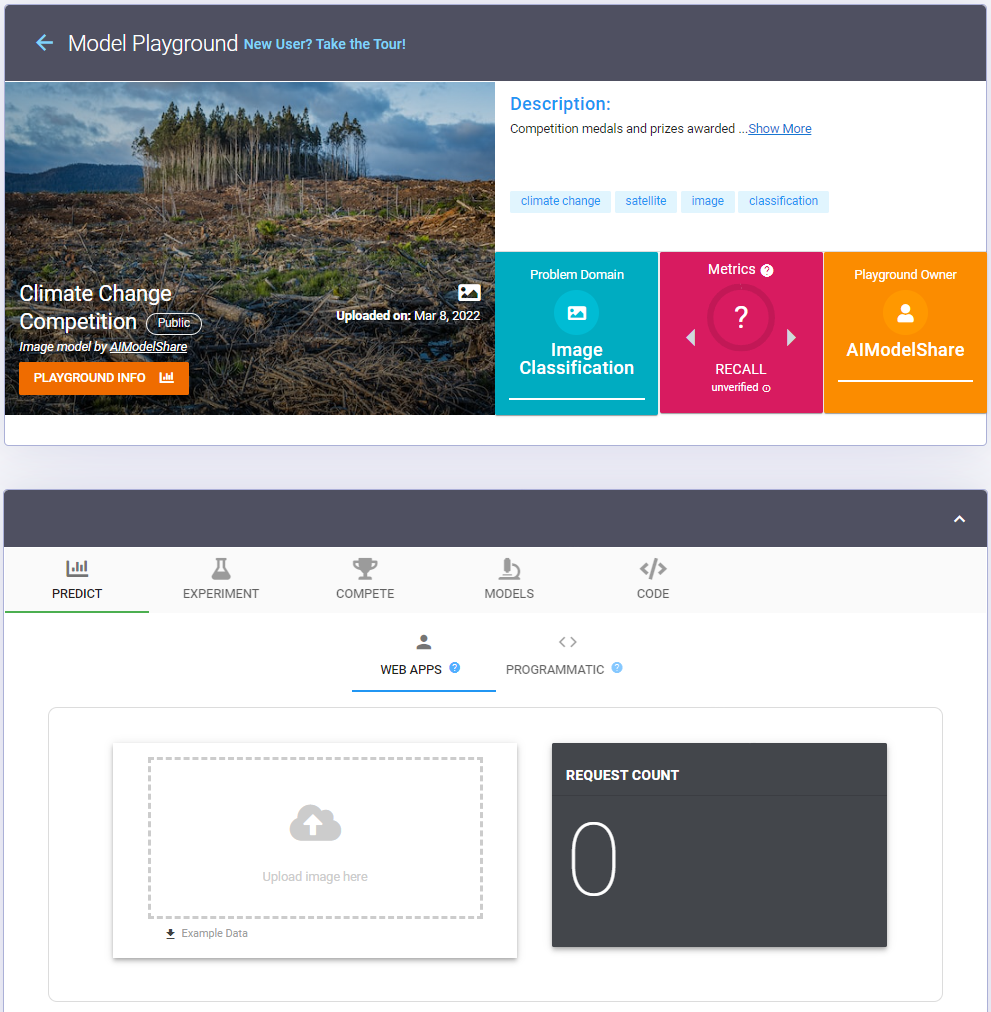
\includegraphics[width=1\textwidth]{figures/playground.png}
  \caption{Example of a Model Playground page. The model playground page allows users to make predictions by uploading data or accessing rebuilt code to make API calls, access Experiment and Competition leaderboards, inspect and compare model architectures, and access code submissions.}
\end{figure}

\newpage
\subsection{D) Example of Competition Leaderboard}
\label{app:competition}

\begin{figure}[h!]
  \centering
  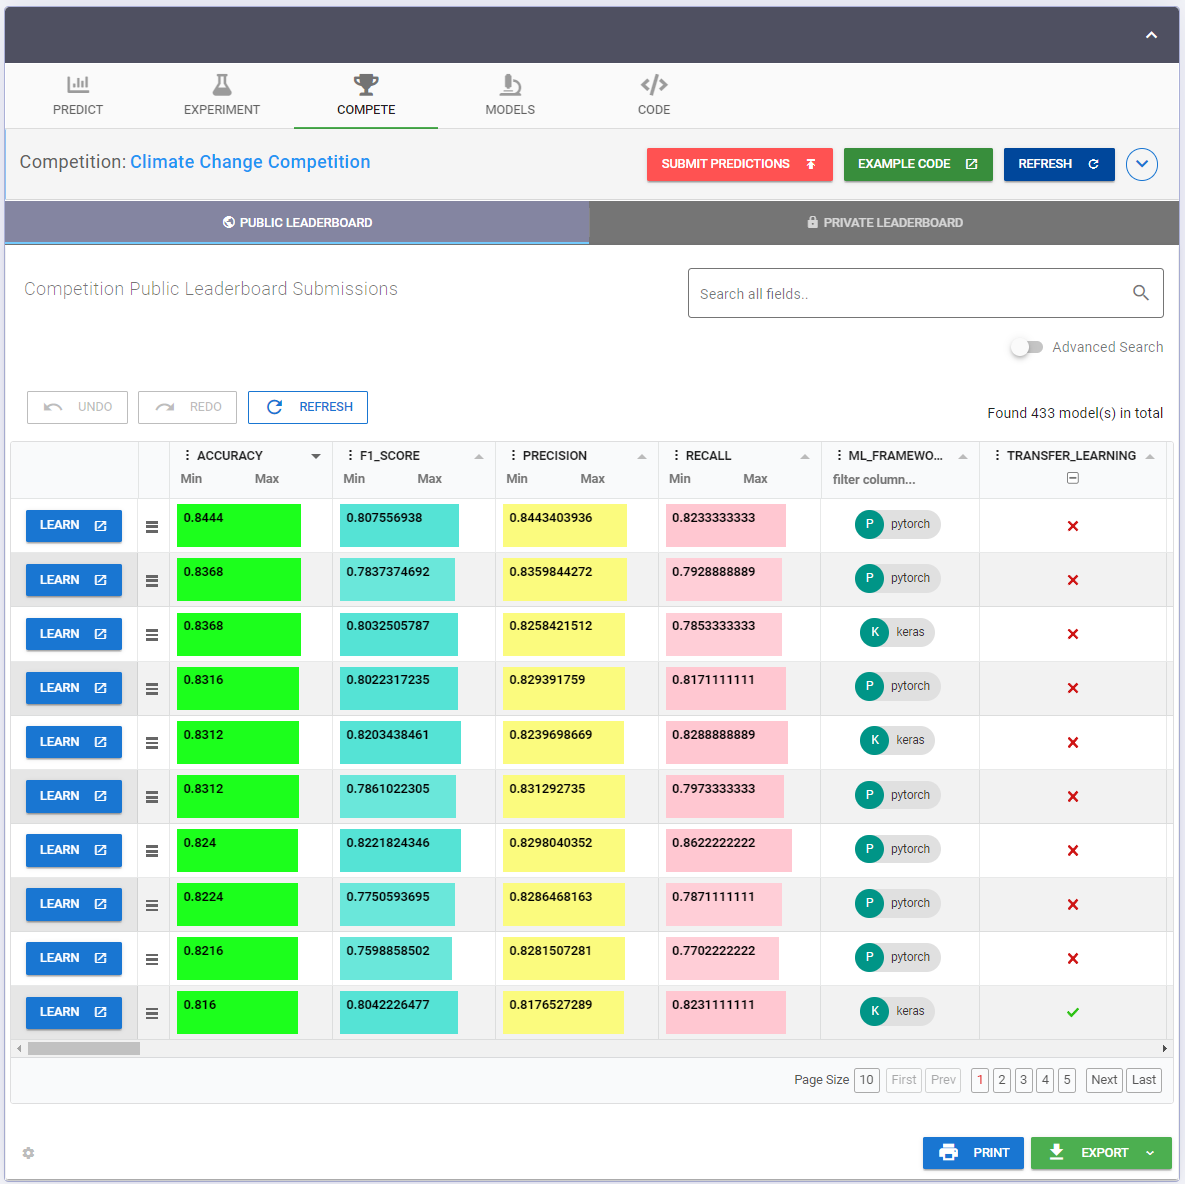
\includegraphics[width=1\textwidth]{figures/competition.png}
  \caption{Example of a Competition Leaderboard. Models submitted to Experiments or Competitions are automatically evaluated and can be ranked according to their evaluation metrics. Model metadata, such as hyperparameter settings, layer types, and dimensions, are depicted in the table (not visible in the screenshot). In order to inspect individual models, users can click on "Learn", which will take them to a Model Details page.}
\end{figure}


\newpage
\subsection{E) Example of Model Details Page}
\label{app:model}

\begin{figure}[h!]
  \centering
  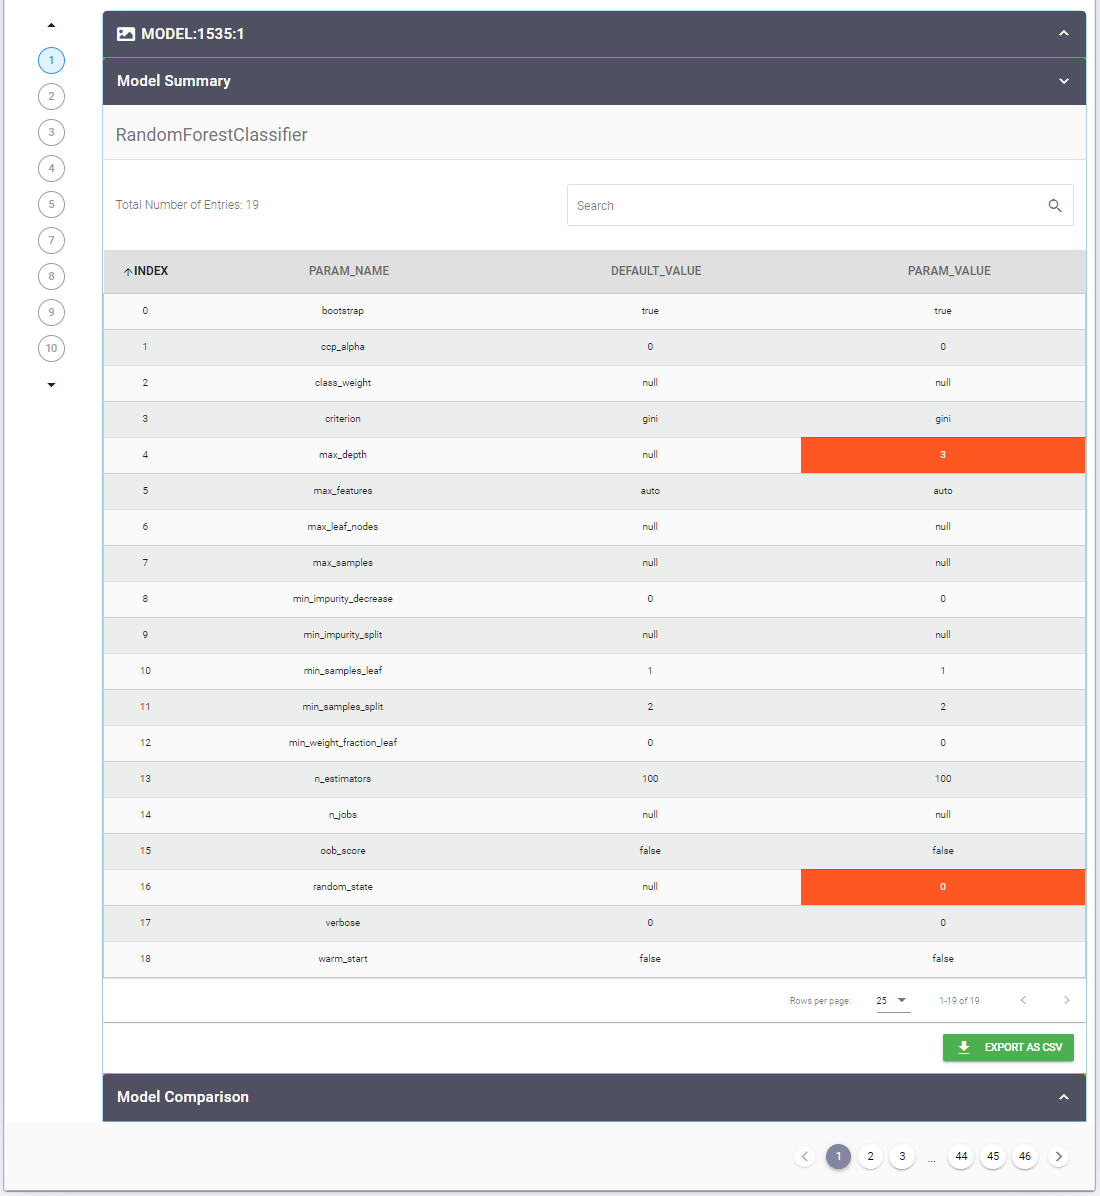
\includegraphics[width=1\textwidth]{figures/model.png}
  \caption{Example of a model and its hyperparameter settings. Users can inspect the hyperparameter settings and model architectures of any model submitted to an Experiment or a Competition.}
\end{figure}